\documentclass{article}

\usepackage{graphicx}
\usepackage[utf8]{inputenc}
\usepackage[T1]{fontenc}
\usepackage[francais]{babel}
\usepackage{hyperref}
\usepackage{amsmath,amsfonts,amssymb}
\usepackage{Tkz-Tab}
\usepackage{wrapfig}
\usepackage{Verbatim}

\begin{document}

\title{L'algue tueuse
	\smallbreak
	TD n\degre3
	\smallbreak
	Modélisation mathématique
	\smallbreak
	Q4}
\author{Sibylle Roux \and Juliette Arazo \and Nicolas Le Gallo \and Tanguy Thomas}


\maketitle

\newpage

\tableofcontents

\newpage

\section{Etude du modèle logistique avec effet Allee et immigration}

\subsection{Etude numérique}

\subsubsection{Modèle avec variation de I}

\paragraph{Courbes de la vitesse d'accroissement}
\begin{center}
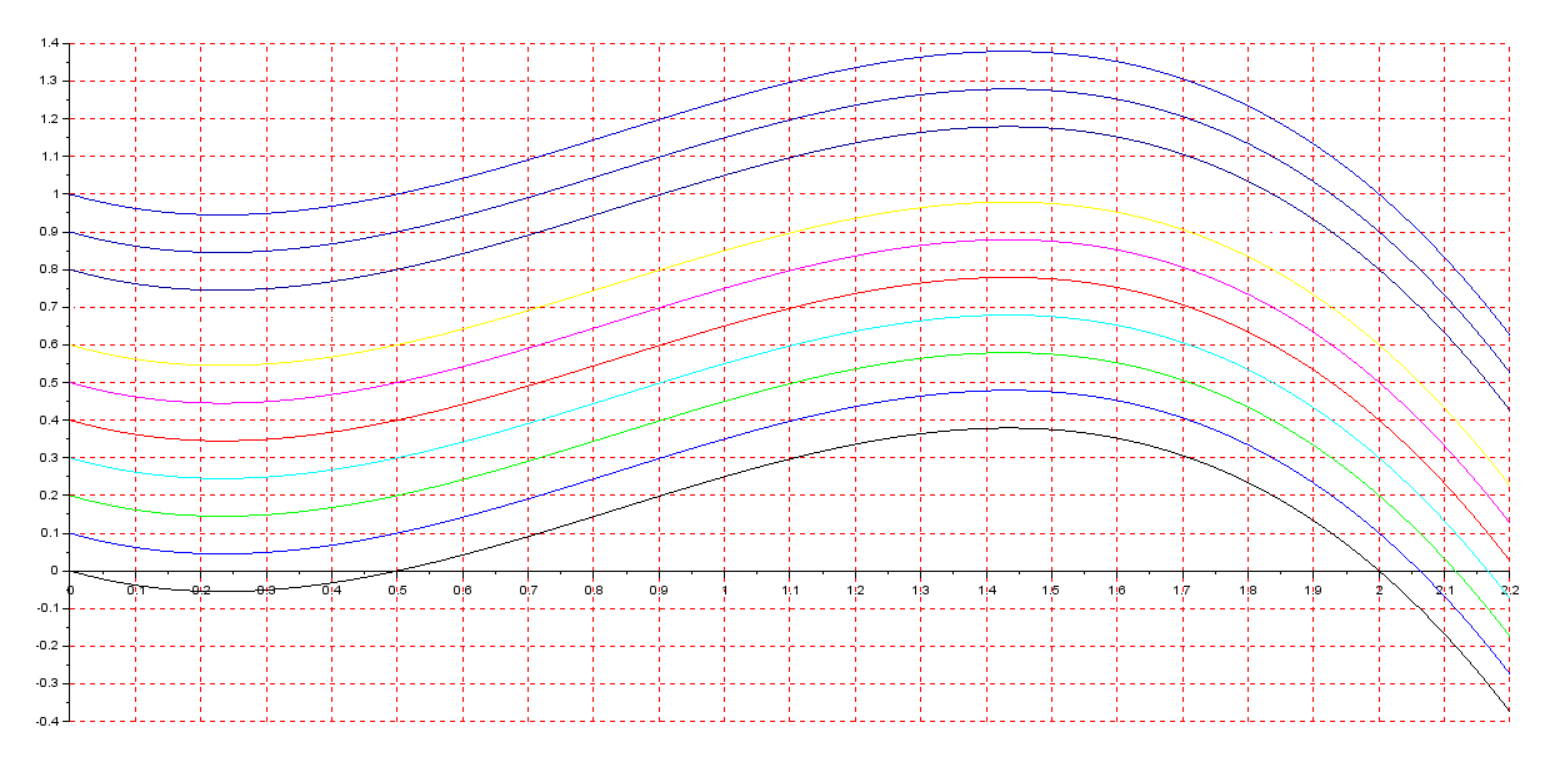
\includegraphics[width=300px]{img/part1/AlleeI.png}
\end{center}
Paramètres de modélisation : $K=2$  ; $r=0.5$ ; $A=0.5$ ; $I$ varie de 0 à 1 avec un pas de 0.1 
\paragraph{}
Sur ce graphique on peut voir les différentes courbes de la vitesse d'accroissement pour différentes valeurs de $I$. On peut voir que les variations de $I$ augmentent la vitesse d'acroissement de manière constante, cela influt donc aussi sur les points d'équilibres du modèle, en effet on voit bien que pour différentes valeurs de I, les points d'équilibres se déplacent sur la courbe, bien que les notions de stabilités/instabilités ne changent pas.
\paragraph{}
On remarque que avec un $I$ assez grand, l'effet Allee n'éteint plus la population mais ralentit seulement sa croissance. En effet 2 points d'équilibres peuvent disparaïtre à partir d'une valeur de I assez grande. Il ne reste donc plus qu'un seul point d'équilibre pour n'importe quelle valeur de population, il correspond à la capacité de charge du modèle (elle ne dépend plus que de $K$ mais aussi de $I$).
\newpage

\paragraph{Discrétisation du modèle}
\begin{center}
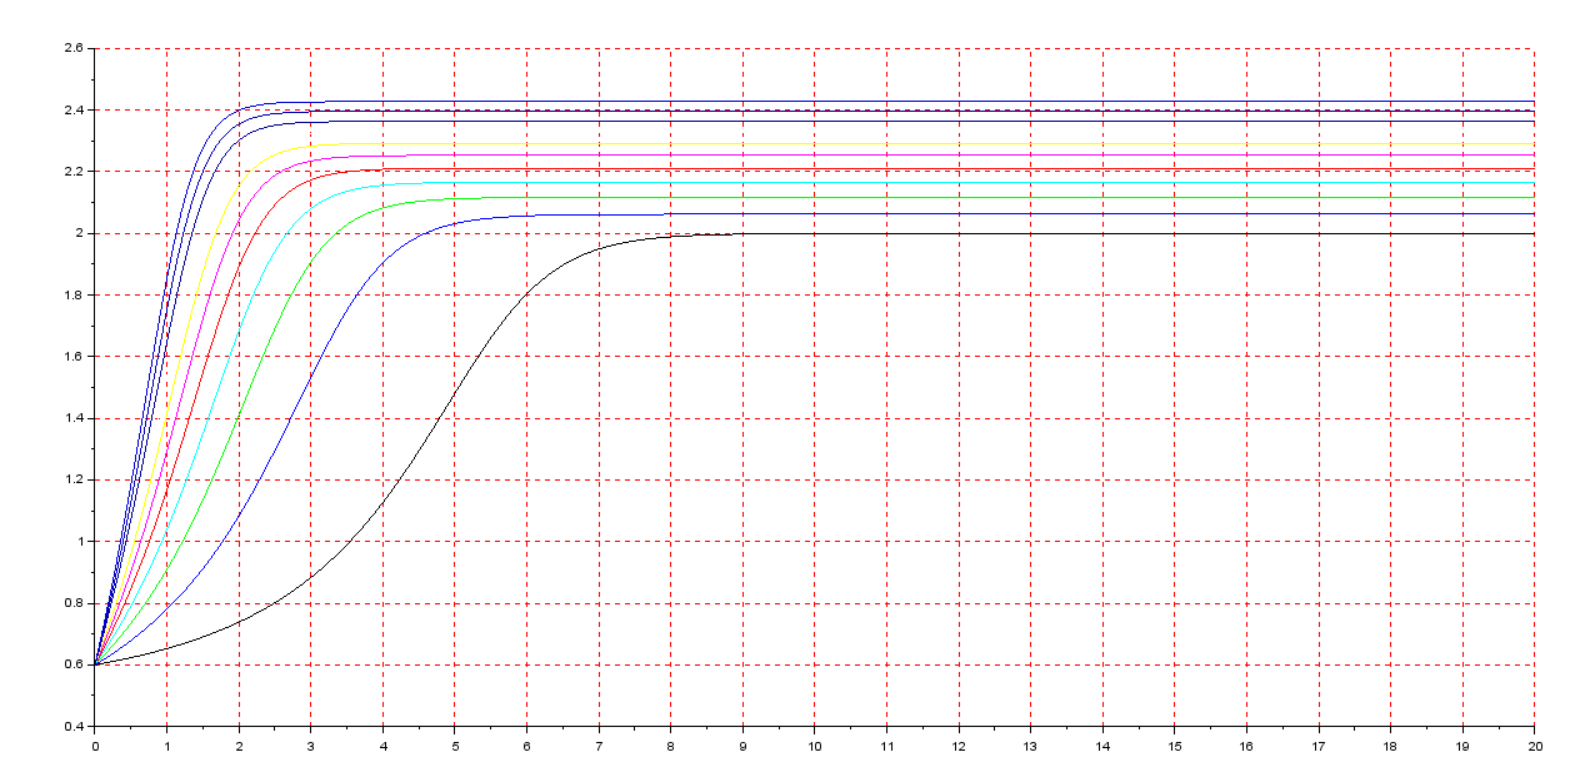
\includegraphics[width=300px]{img/part1/TrajI.png}
\end{center}
Paramètres de modélisation : $a=0.6$ ; $K=2$  ; $r=0.5$ ; $A=0.5$ ; $I$ varie de 0 à 1 avec un pas de 0.1
\paragraph{}
Sur ces courbes, on remarque bien que les variations de $I$, influent sur la capacité de charge du modèle, ainsi que la vitesse à laquelle il l'atteint.

\subsubsection{Modèle avec variation de K}

\paragraph{Courbes de la vitesse d'accroissement}
\begin{center}
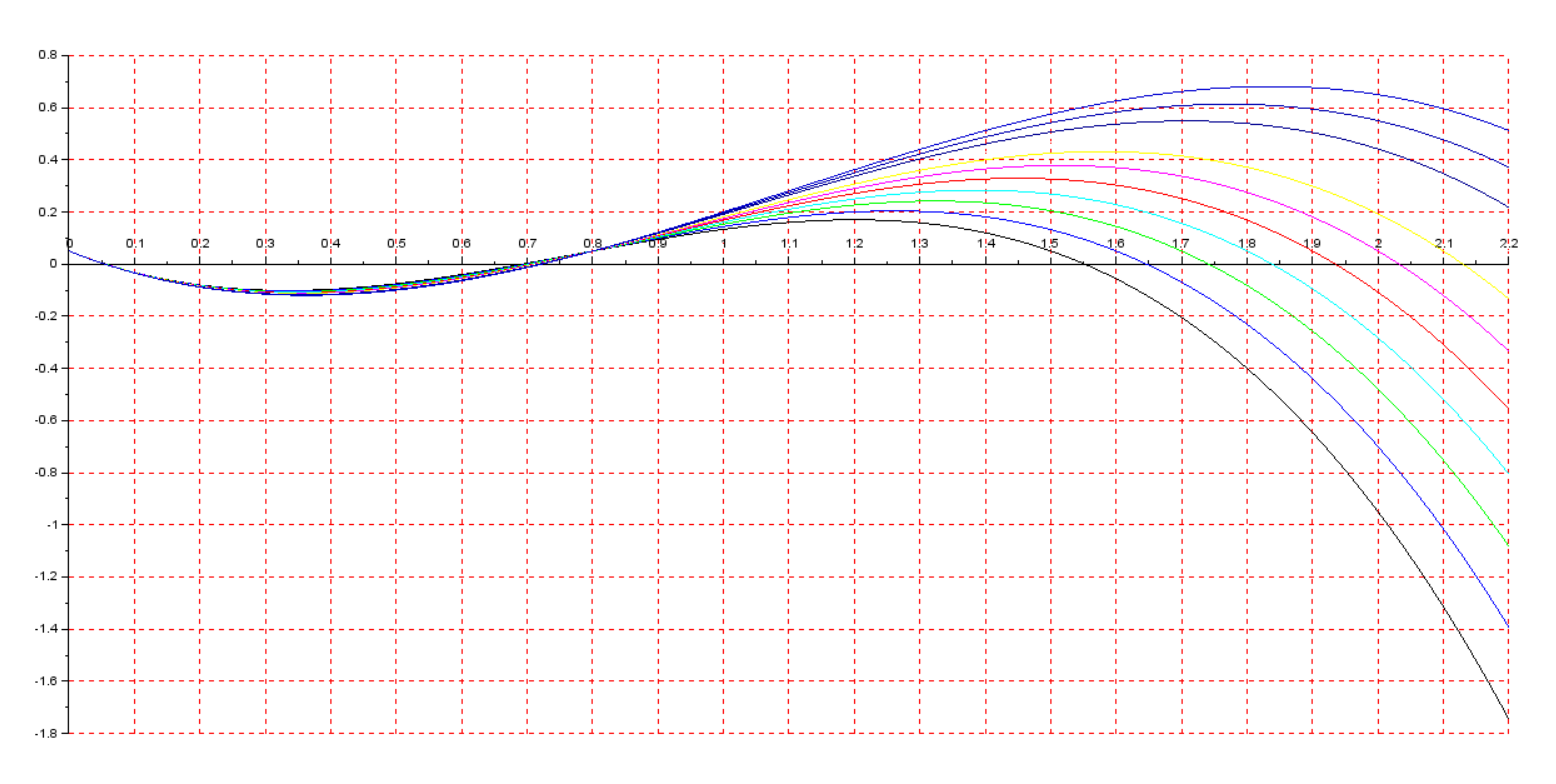
\includegraphics[width=300px]{img/part1/AlleeK.png}
\end{center}
Paramètres de modélisation : $r=1$ ; $A=0.8$ ; $I=0.05$ ; $K$ varie de 1.5 à 2.5 avec un pas de 0.1
\paragraph{}
Sur ce graphique on remarque que les variations de $K$ ont le même effet que sur le modèle logistique avec effet Allee. Les variations de $K$ déterminent la capacité de charge du modèle ($I$ influt aussi dans la capacité de charge). On remarque juste que le premier point d'équilibre stable (celui vers $0.05$, on l'appellera $E1$) permet à la population de ne jamais completement s'éteindre mais de tendre vers cette valeur.
On remarque donc que 2ème point d'équilibre (on l'appellera $E2$), celui instable vers $0.7$ est une valeur séparatrice des 2 bassins d'attractions :
\begin{itemize}
\item Lorsque la population initiale est inférieure à $E2$, la population va tendre vers l'équilibre stable $E1$,
\item Lorsque la population initiale est supérieure à $E2$, la population va tendre ves sa capacité de charge.
\end{itemize}

\paragraph{Discrétisation du modèle}
\begin{center}
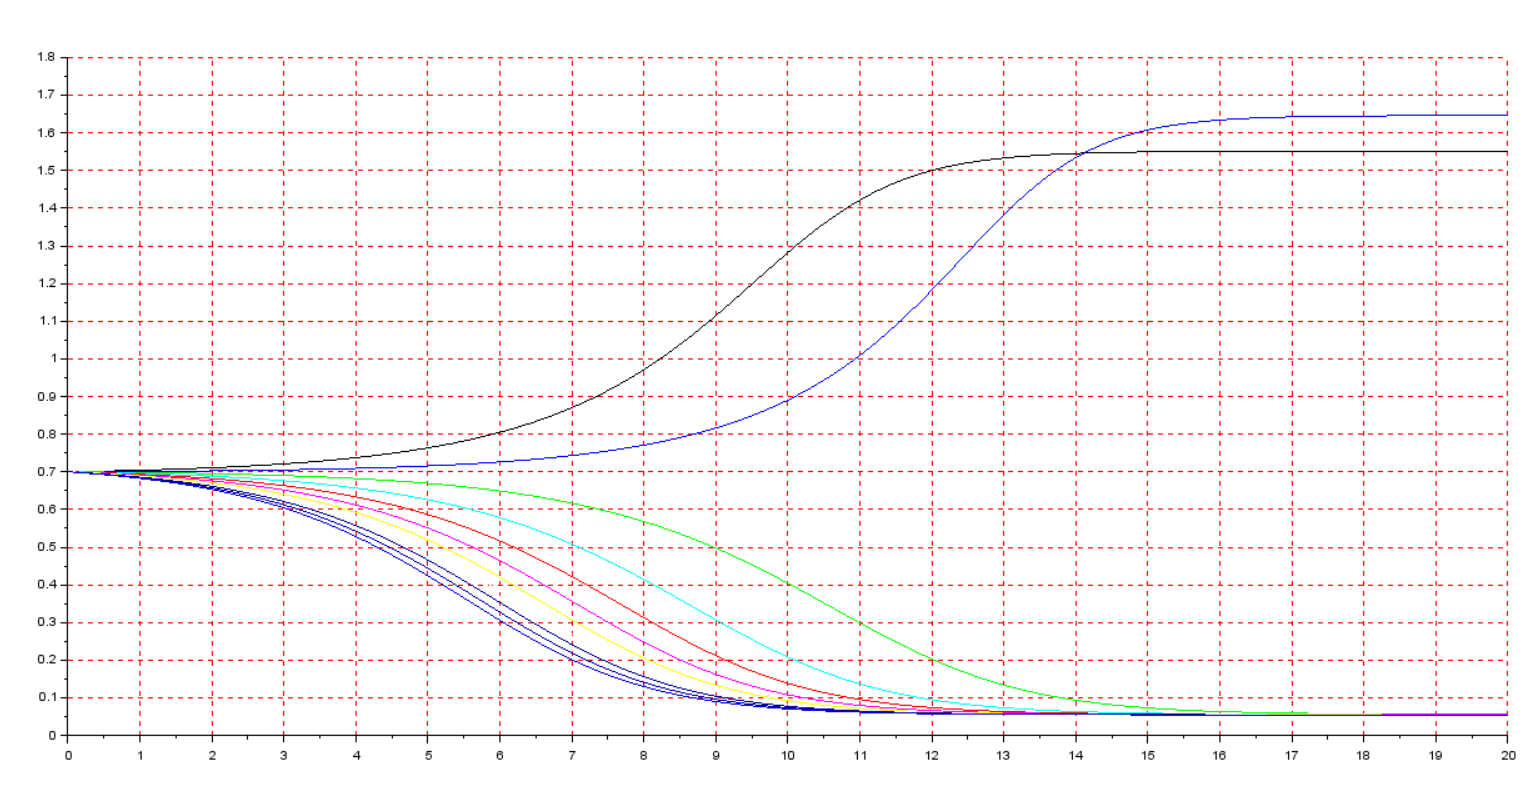
\includegraphics[width=300px]{img/part1/TrajK.png}
\end{center}
Paramètres de modélisation : $a=0.7$ ; $r=1$ ; $A=0.8$ ; $I=0.05$ ; $K$ varie de 1.5 à 2.5 avec un pas de 0.1
\paragraph{}
Sur ce graphique nous avons pris $a=0.7$, or sur le dernier graphique on voit bien que la valeur séparatrice $E2$ est proche de $0.7$. C'est pour cela que l'on peut voir les 2 bassins d'attractions du modèle, ici :
\begin{itemize}
\item On remarque que 2 courbes tendent vers leurs capacité de charge respective,
\item Mais que les autres courbes tendent vers le point d'équilibre stable $E1$.
\end{itemize}

\newpage

\subsubsection{Modèle avec variation de A}

\paragraph{Courbes de la vitesse d'accroissement}
\begin{center}
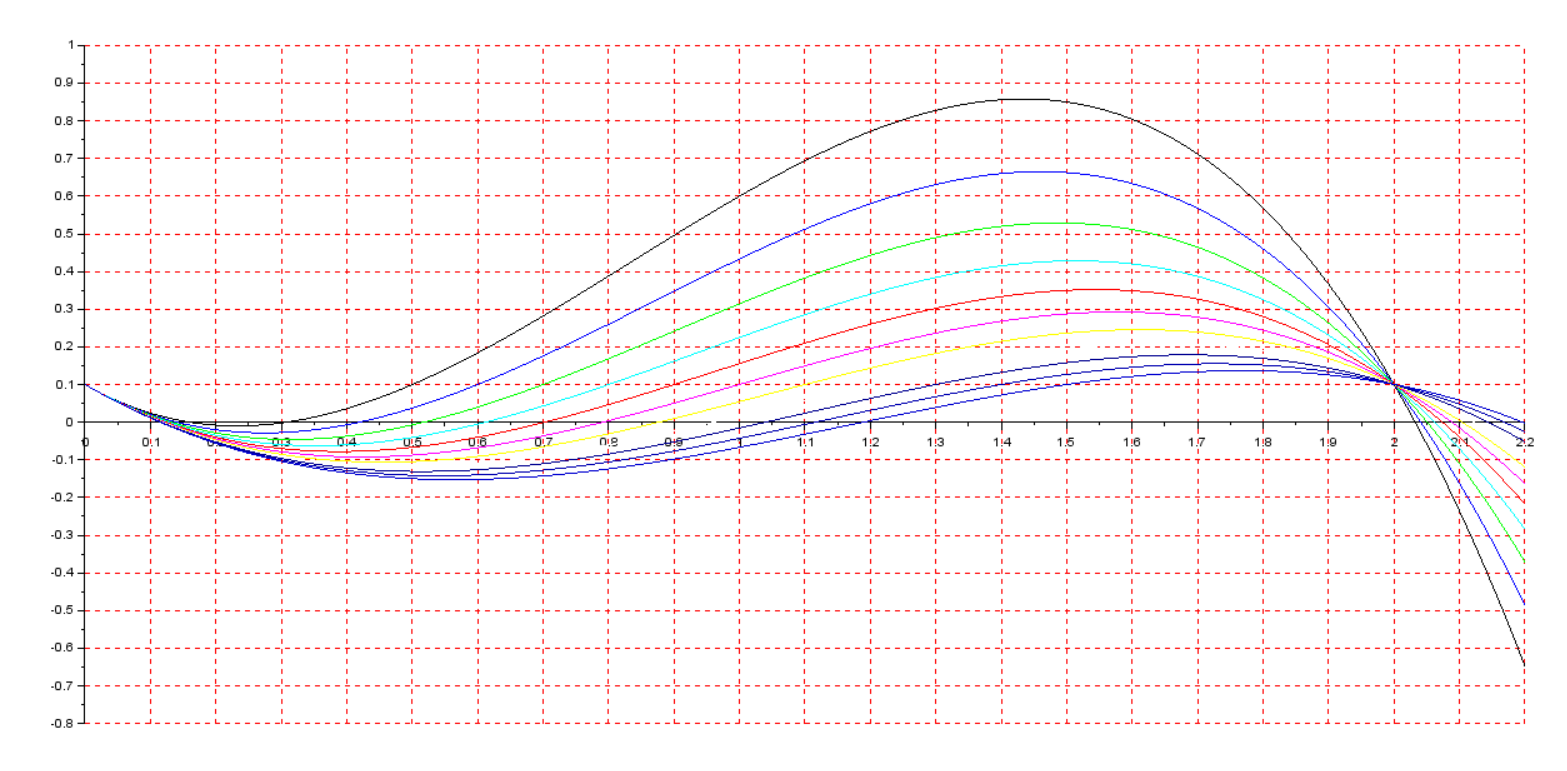
\includegraphics[width=300px]{img/part1/AlleeA.png}
\end{center}
Paramètres de modélisation : $I=0.1$ ; $K=2$ ; $r=1$  ; $A$ varie de 0.5 à 1.5 avec un pas de 0.1
\paragraph{}
Sur ce graphique on remarque bien que $A$ influt sur la valeur séparatrice du modèle, en effet les variations de $A$ permettent de changer la position de ce point d'équilibre, ainsi donc que la taille des 2 bassins d'attractions.

\paragraph{Discrétisation du modèle}
\begin{center}
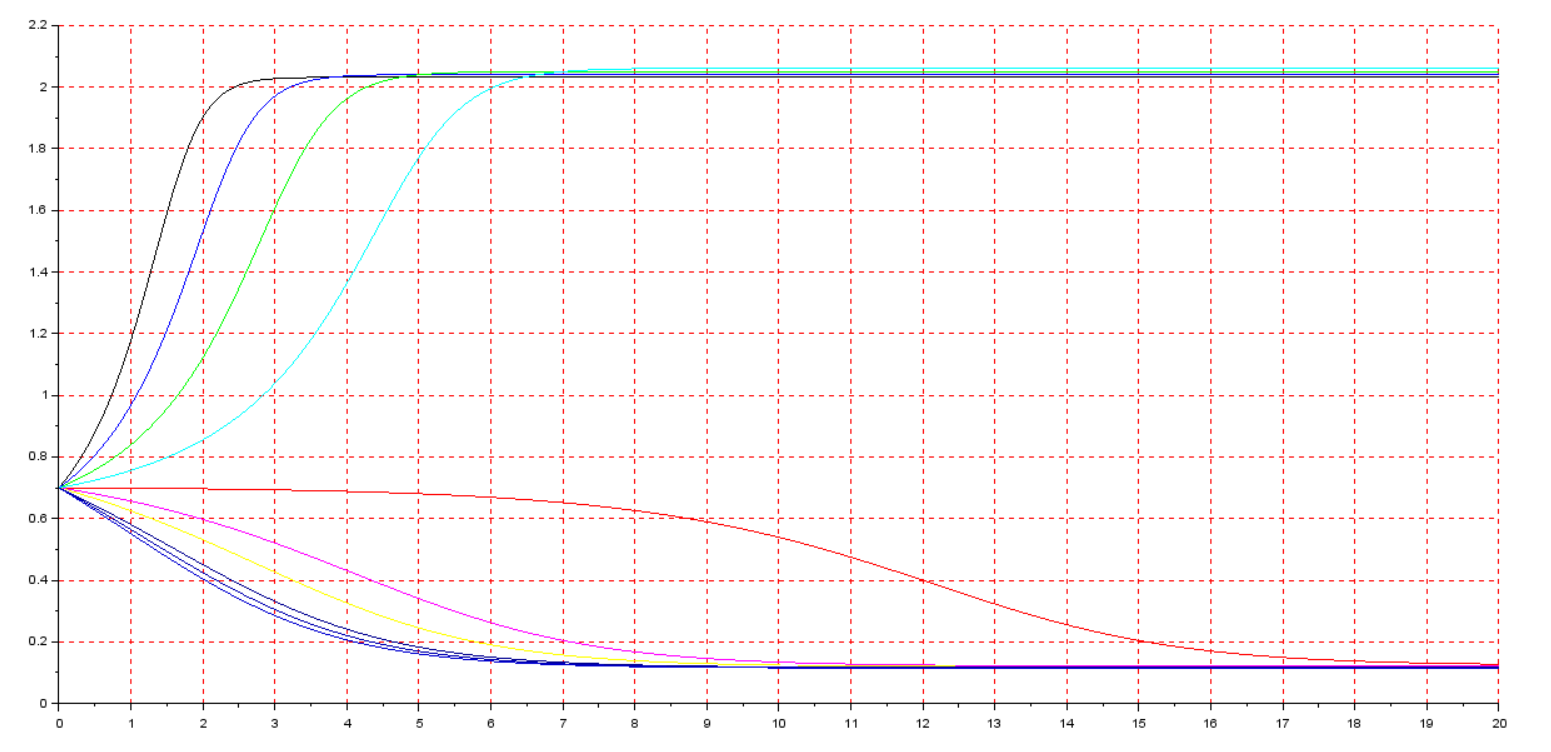
\includegraphics[width=300px]{img/part1/TrajA.png}
\end{center}
Paramètres de modélisation : $a=0.7$ ; $I=0.1$ ; $K=2$ ; $r=1$  ; $A$ varie de 0.5 à 1.5 avec un pas de 0.1
\paragraph{}
A partir de ces courbes avec la même population initiale : $a=0.7$, on voit que pour les différentes valeurs de $K$, les courbes tendent vers :
\begin{itemize}
\item la capacité de charge du modèle si $E2 > a$
\item $E1$ si $E2<a$
\item $E2$ si $a=E2$
\end{itemize}

\subsubsection{Modèle avec variation de la population initiale}

\paragraph{Discretisation du modèle}
\begin{center}
\includegraphics[width=300px]{img/part1/TrajPop.png}
\end{center}
Paramètres de modélisation : $A=0.5$ ; $I=0.05$ ; $K=2$ ; $r=0.5$  ; $a$ varie de 0.2 à 2.2 avec un pas de 0.2
\paragraph{}
Sur ce graphique on fait varier $a$ de manière à voir les 2 points d'équilibres stables du modèle. On remarque que pour la courbe qui démarre à $0.2$, la courbe tend vers $E1$, et les autres courbes vers $E3$.

\newpage

\subsection{Etude mathématique}

Comme nous l'avons vu dans le TD précédent, l'effet Allee possède 3 points d'équilibres : 

\begin{align}
x’(t) = f(x) = r \times x \times (\frac{x}{A} - 1) \times (1 - \frac{x}{K}) + I
\intertext{Avec $0<A<K$}
x’(t) = f(x) = r \times x \times (\frac{x}{A} - 1) \times (1 - \frac{x}{K}) + I \\
f(x) =  \frac{r \times x^{2}}{A} - \frac{r \times x^3}{A \times K} - r \times x+ \frac{r \times x^2}{K} + I
\intertext{Calculons x"'(t) = f'(x) :}
f'(x) = \frac{r \times 2 \times x\times A}{A^2} - \frac{r \times 3 \times x^2 \times A \times K}{(A \times K)^2} - \frac{r \times A \times K}{A \times K} + \frac{r \times 2 \times x \times K}{K^2}
\intertext{Après factorisation :}
f'(x) = -3 \times x^2 + 2 \times x \times (K+A) - A \times K =0
\intertext{Calcul des racines :}
Delta = 4 \times (A+K)^2 - 4 \times -3 \times (- A \times K) \\
Delta = 4 \times (A^2+K^2-A \times K)
\end{align}

\begin{center}
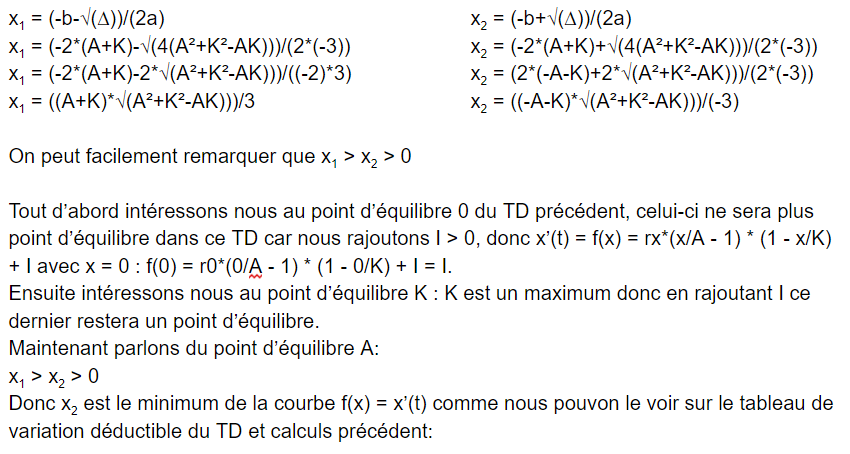
\includegraphics[width=400px]{1.png}
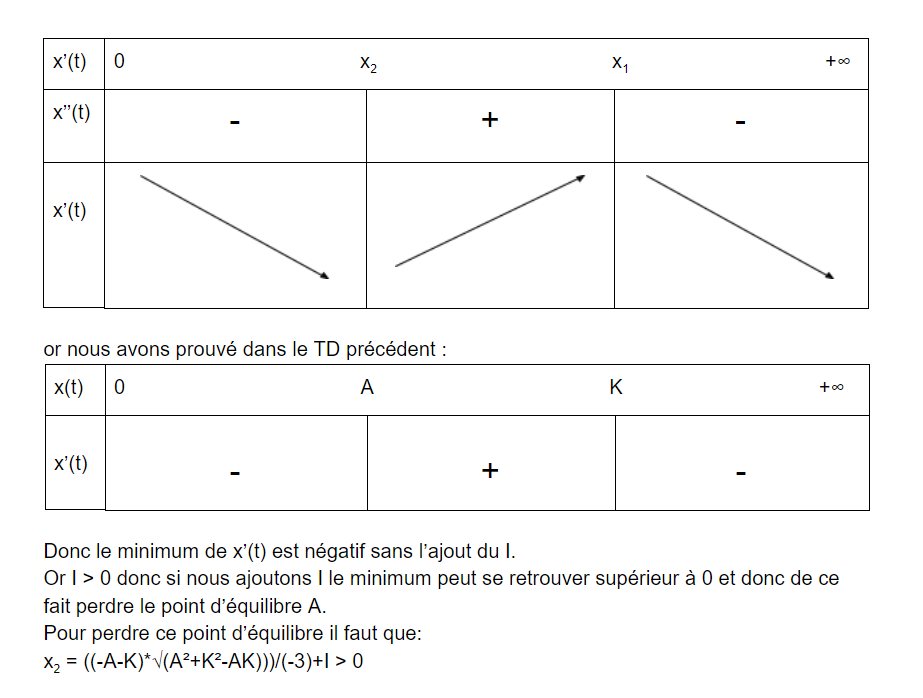
\includegraphics[width=400px]{2.png}
\end{center}

\subsection{Bilan}
\paragraph{}

\newpage
\section{Etude du modèle logistique avec prédation}

\subsection{Etude numérique}

\subsubsection{Modèle}

\paragraph{Vitesse d'accroissement}
\begin{center}
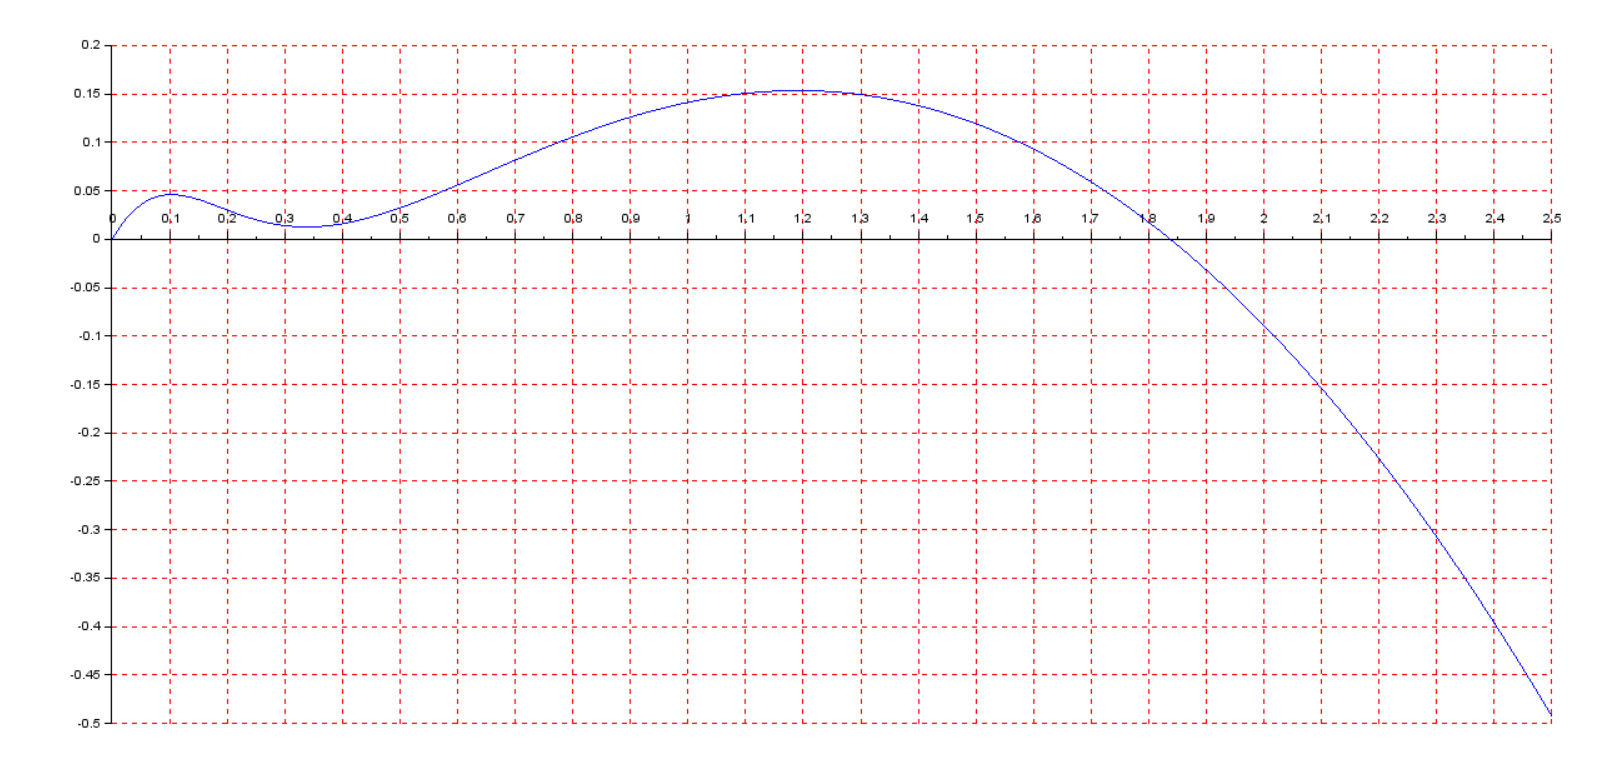
\includegraphics[width=300px]{img/part2/Log.png}
\end{center}
Paramètres de modélisation : $r=1$ ; $A=0.5$ ; $K=2.5$ ; $B=0.5$ ; $C=0.3$
\paragraph{}
Ce graphique est la représentation de la vitesse d'accroissement du modèle logistique avec effet de prédation.
On remarque que lorsque la population atteint la valeur de C (ici 0,3), sa vitesse d'accroissement diminue beaucoup: on constate ici l'influence de C, qui représente la valeur de la population à partir de laquelle la prédation va entrer en jeu.
On peut aussi sur cette courbe 2 points d'équilibre, l'un instable et l'autre stable, respectivement : 0 et 1.838 .
On remarque finalement que la population n'atteint jamais sa capacité de charge, étant donné qu'elle est constamment soustraite par un facteur positif $( B * (x\up{2} +C\up{2}))$.

\paragraph{Discretisation}
\begin{center}
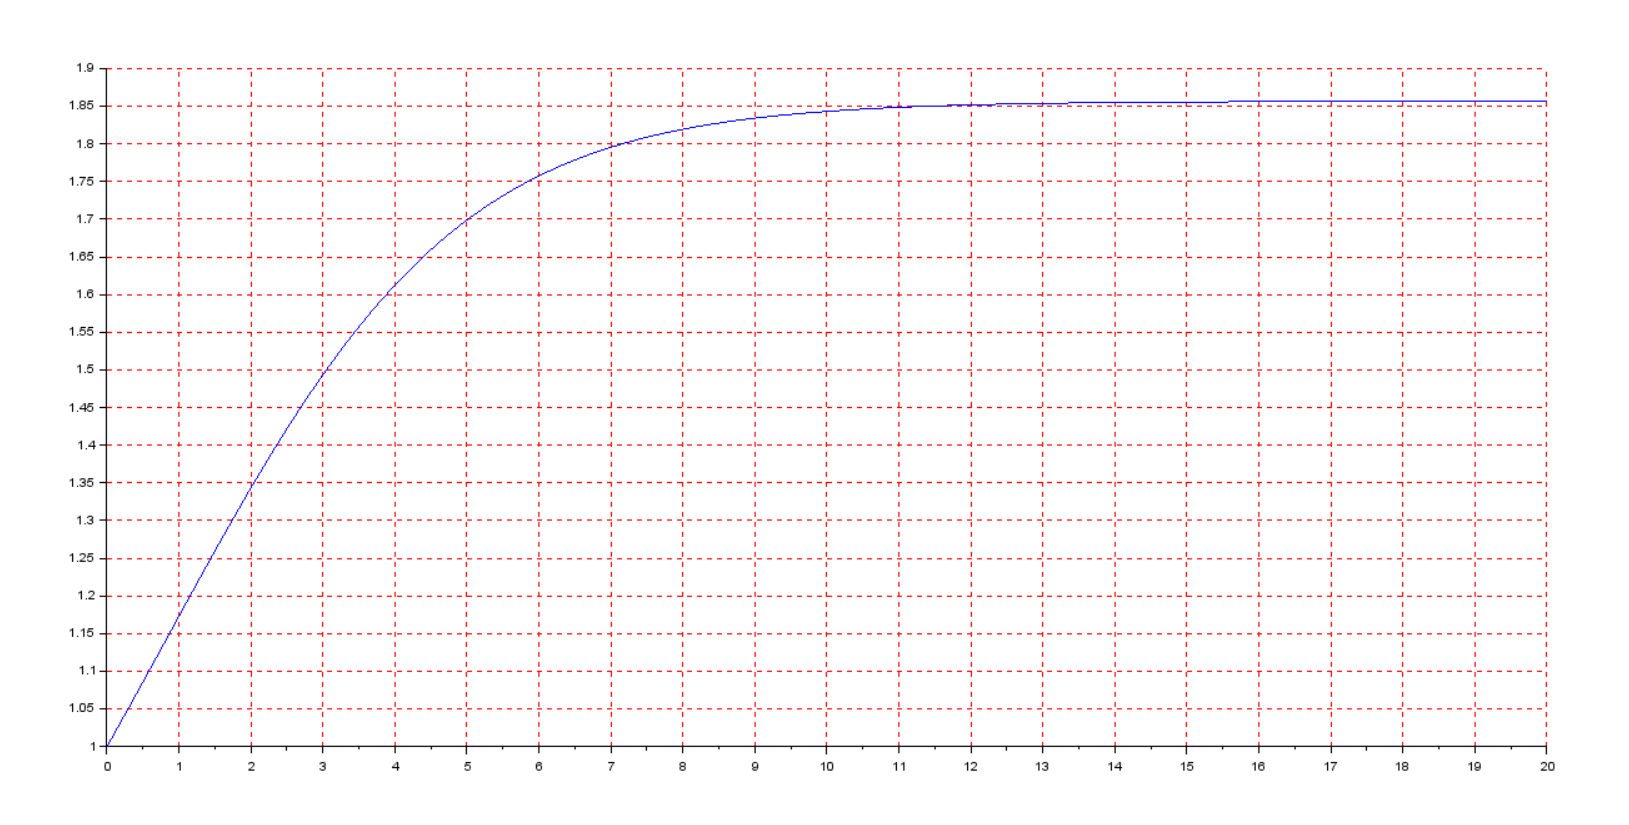
\includegraphics[width=300px]{img/part2/Traj.png}
\end{center}
Paramètres de modélisation : $r=1$ ; $A=0.5$ ; $K=2.5$ ; $B=0.5$ ; $C=0.4$ ; $h=0.05$ ; $a=1$
\paragraph{}
Ce graphique nous montre l'évolution de la population en fonction du temps, d'après le modèle logistique avec effet de prédation. On observe une trajectoire en S, comme pour le modèle logistique classique, à la seule différence qu'ici le potentiel de charge K n'est jamais atteint car la population totale est toujours soustraite par le même facteur positif, elle tend ainsi vers son point d'équilibre ( stable).

\subsubsection{Modèle avec variation de B}

\paragraph{Vitesse d'accroissement}
\begin{center}
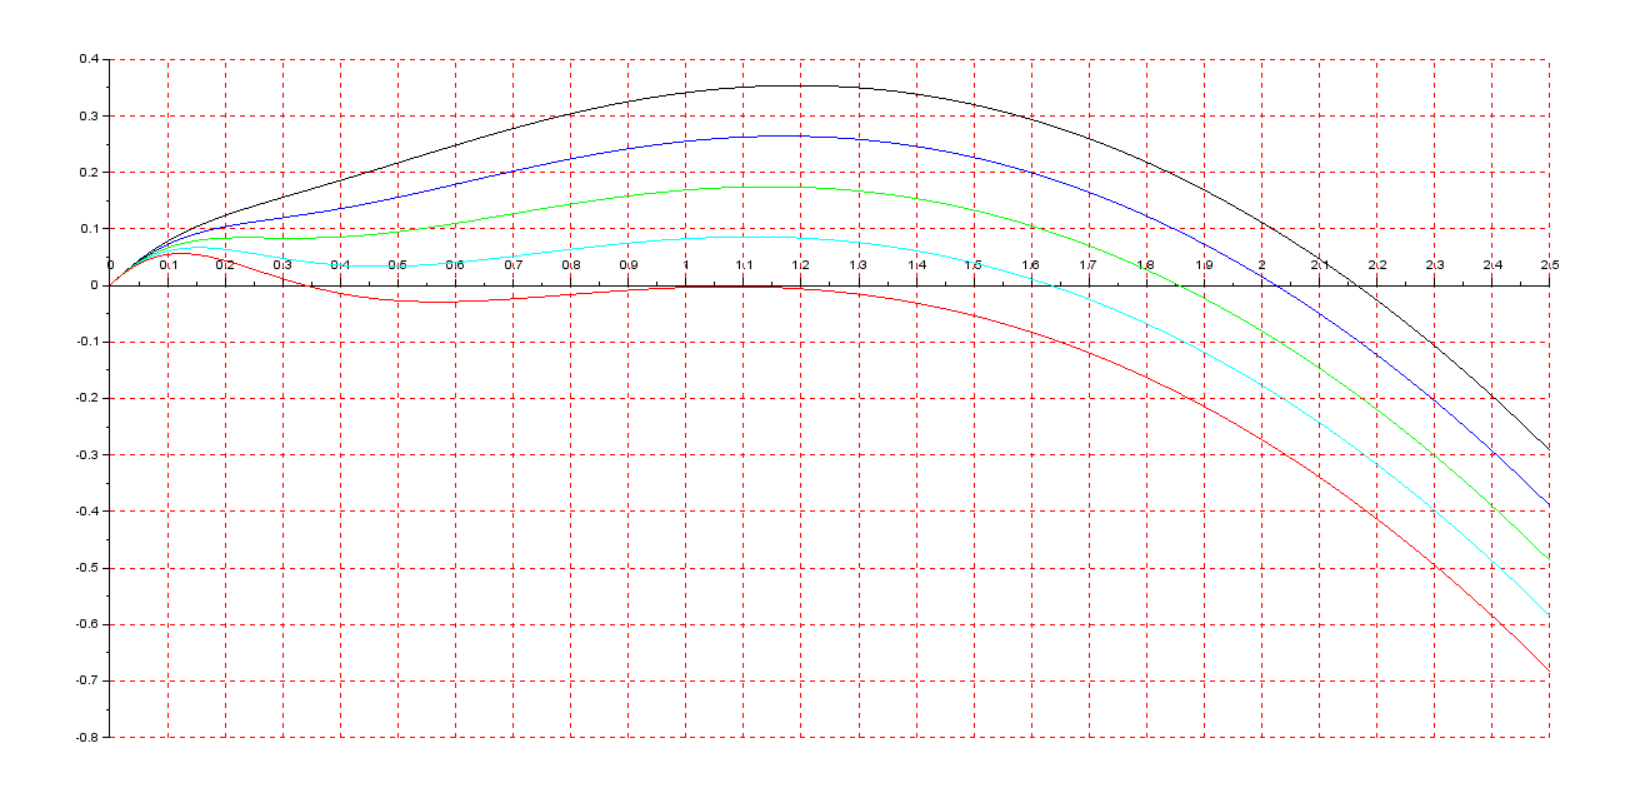
\includegraphics[width=300px]{img/part2/LogB.png}
\end{center}
Paramètres de modélisation : $r=1$ ; $A=0.5$ ; $K=2.5$ ; $C=0.4$ ; $B$ varie de 0.3 à 0.7 avec un pas de 0.1
\paragraph{}
Ce graphique représente le taux d'accroissement d'une population selon le modèle logistique avec effet de prédation, avec une variation du paramètre B. On observe donc plusieurs courbes qui nous permettent d'affirmer les choses suivantes: plus B est petit, moins la population totale est impactée par la perte d'individu, et plus son accroissement se rapproche de celle du modèle logistique. Inversement, plus B est grand plus l'acroissement va être faible et l (même négatif à partir du moment où la prédation est déclenchée ) et la population va être faible.    Comme pour le taux d'accroissement de base, on observe deux points d'équilibres, l'un instable et l'autre stable, pour toutes les courbes. Cependant le point d'équilibre stable n'est pas atteint à la même valeur pour chaque courbe.

\paragraph{Discretisation}
\begin{center}
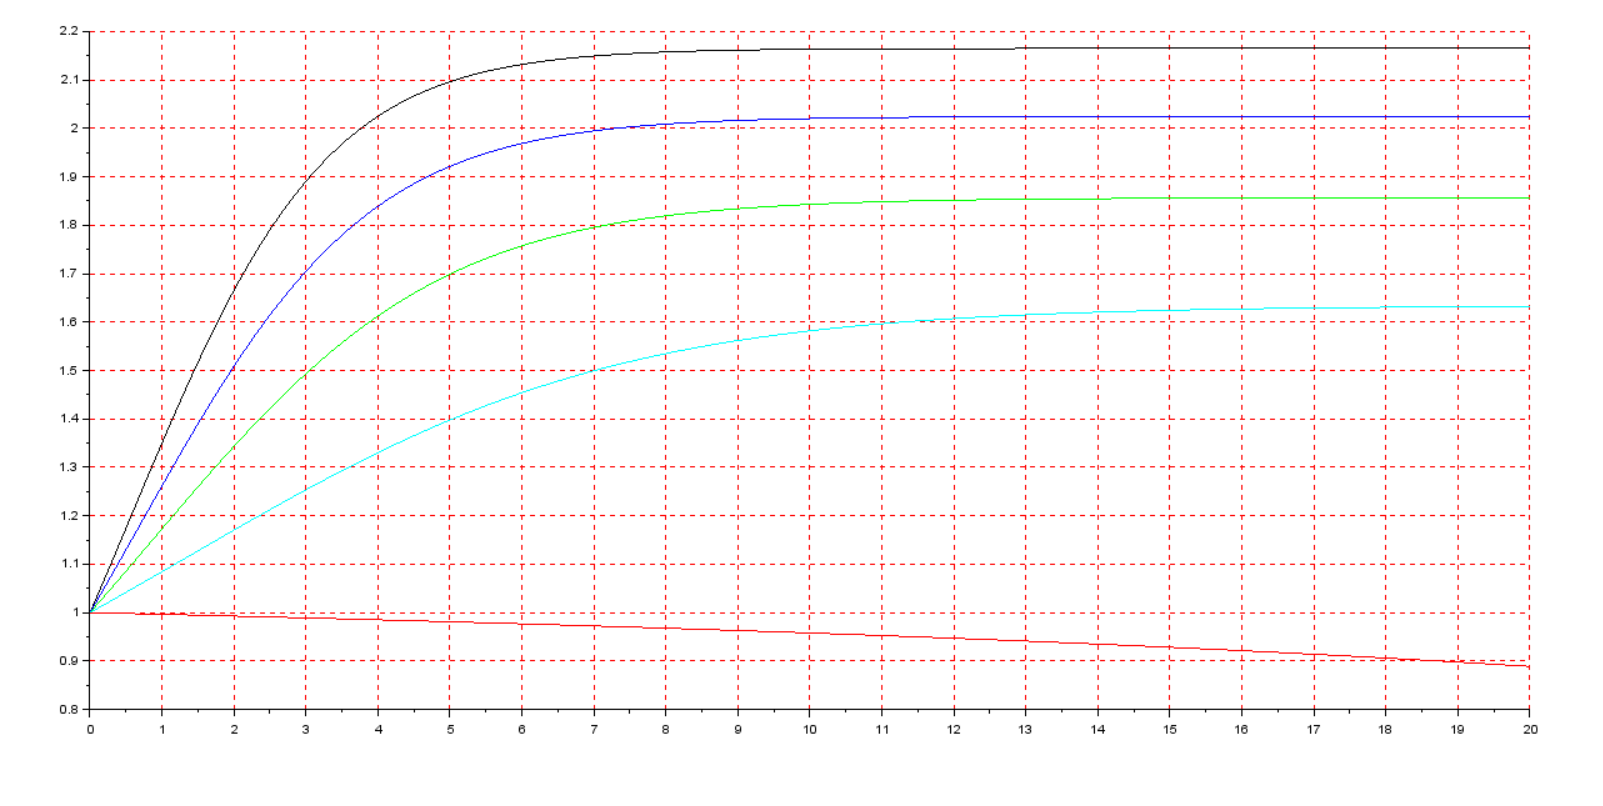
\includegraphics[width=300px]{img/part2/TrajB.png}
\end{center}
Paramètres de modélisation : $r=1$ ; $A=0.5$ ; $K=2.5$ ; $C=0.4$ ; $h=0.05$ ; $a=1$ ; $B$ varie de 0.3 à 0.7 avec un pas de 0.1
\paragraph{}
Ce graphique nous montre la trajectoire de la population selon le modèle logistique avec effet de prédation, avec une variation de la variable B. Comme remarqué pour la variation de B sur le taux d'accroissement, plus B est petit plus la population augmente et augmente vite,vers son point d'équilibre (différent pour chaque courbe comme vu pour le taux d'accroissement correspondant ) . Inversement, on remarque que lorsque B est grand, la population décroît et se stabilise à une valeur légèrement inférieure à 0,9.

\subsubsection{Modèle avec variation de C}

\paragraph{Vitesse d'accroissement}
\begin{center}
\includegraphics[width=300px]{img/part2/logC.png}
\end{center}
Paramètres de modélisation :  $r=1$ ; $A=0.5$ ; $K=2.5$ ; $B=0.5$ ; $C$ varie de 0.2 à 0.4 avec un pas de 0.05
\paragraph{}
Ce graphique nous montre le taux d'accroissement de la population selon le modèle logistique avec effet de prédation, et avec une variation du paramètre C. Ces différentes courbes nous montrent plus précisément l'impact de C sur le taux d'accroissement: plus C est grand, plus la population nécessaire à la mise en place de la prédation diminue. On observe sur le graphique les courbes pour lesquelles C est grand, l'accroissement devient négatif très rapidement. Pour les courbes avec un petit C, la prédation prend effet plus tard et n'a pas un énorme impact sur l'accroissement de la population car celle-ci est déjà suffisament importante.
\paragraph{}
Pour les deux courbes avec la valeur de C la plus grande, on constate 4 points d'équilibre, successivement instables, stables, instables et stables. On observe aussi 2 bassins d'attractions (autour de 0.2 et 1.8)mais aussi une valeur séparatrice (autour de 0.5).
\paragraph{}
Pour les autres courbes, les points stables sont identiques que pour le taux d'accroissement de base, et le seul bassin d'attraction est celui du maximum de la population.

\paragraph{Discretisation}
\begin{center}
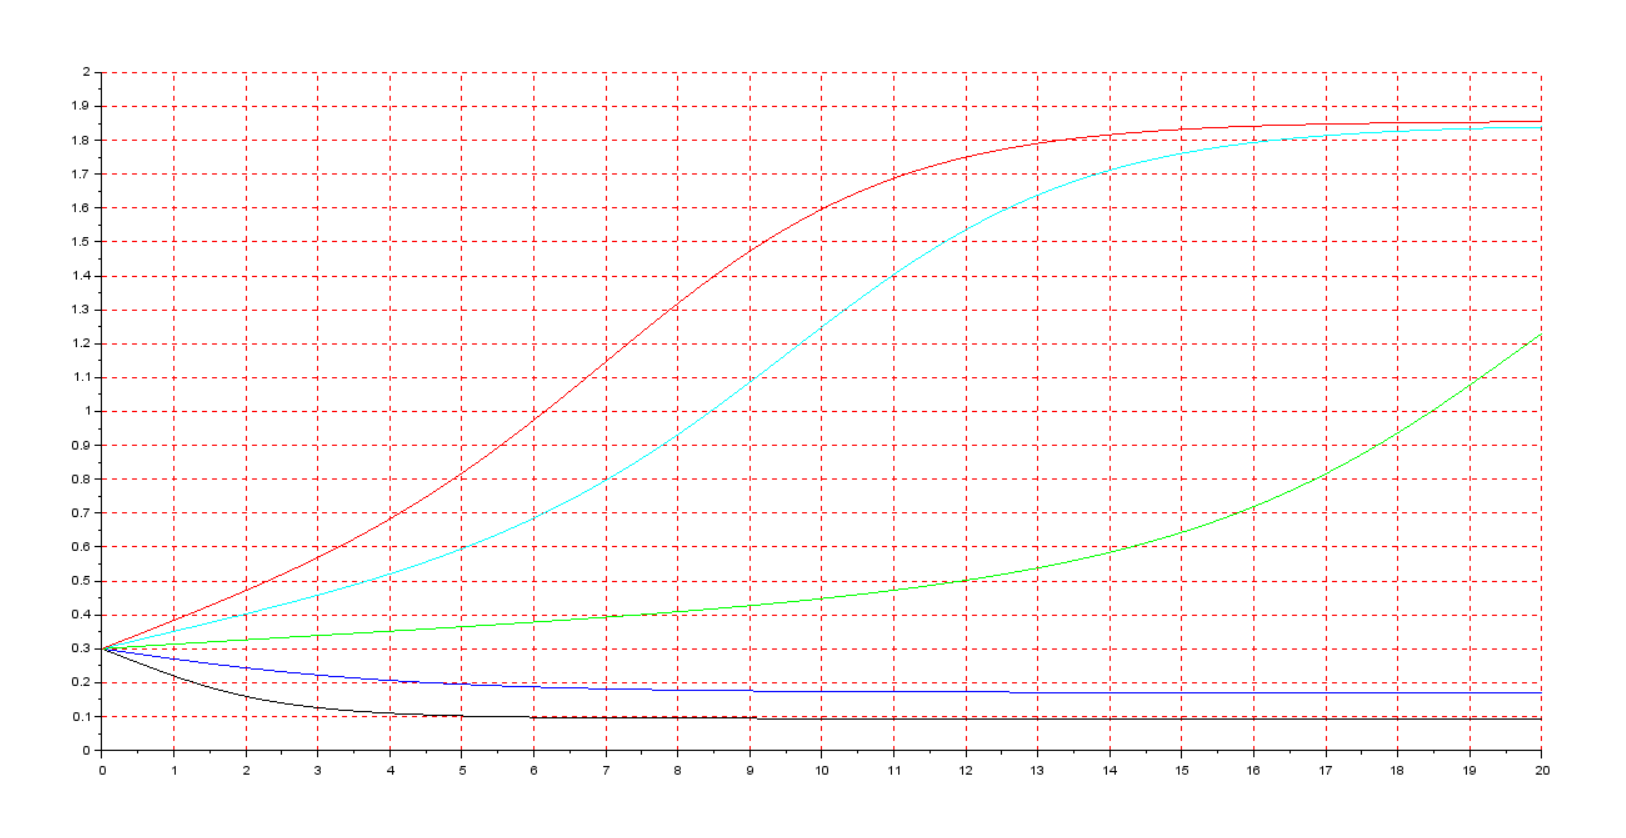
\includegraphics[width=300px]{img/part2/TrajC.png}
\end{center}
Paramètres de modélisation :  $r=1$ ; $A=0.5$ ; $K=2.5$ ; $B=0.5$ ; $h=0.05$ ; $a=0.3$ ; $C$ varie de 0.2 à 0.4 avec un pas de 0.05
\paragraph{}
Ce graphique représente la trajectoire de la population avec une variation du paramètre C.  On voit que plus C est grand, moins la population croît vite, et même pour les valeurs de C les plus grandes la population décroît. Ces courbes nous permettent aussi d'observer certains points d'équilibres, au nombre de 3 : 2 aux extremums, stables, et un au milieu qui est instable et qui est séparateur.Légèrement au dessus de lui, la population va vers le bassin d'attraction du haut, et légèrement en dessous la population va vers le bassin du bas. C'est moins de points d'équilibre que pour le taux d'accroissement correspondant car la population initiale est ici de 0.3, tandis que le taux d'accroissement nous indiquait un autre point d'équilibre entre 0 et 0.3.

\subsubsection{Modèle avec variation de la population initiale}

\paragraph{Discretisation}
\begin{center}
\includegraphics[width=300px]{img/part2/TrajPop.png}
\end{center}
Paramètres de modélisation : $r=1$ ; $A=0.5$ ; $K=2.5$ ; $B=0.5$ ; $h=0.05$ ; $C=0.4$ ; $I=0.2$ ; $a$ varie de 0.5 à 3.5 avec un pas de 0.5
\paragraph{}
Ce graphique nous montre l'évolution de la population d'après le modèle logistique avec effet de prédation, avec le paramètre a ( population initiale) qui varie. On remarque ici l'influence de la population sur la prédation: pour une population très élevèe, celle-ci va décroître très rapidement vers le bassin d'attraction de son point d'équilibre stable. En revanche pour une population petite, la prédation ne va pas avoir beaucoup d'impact et la population va croître rapidement vers le bassin d'attraction de son point d'équilibre stable.

\subsection{Etude mathématique}

\begin{center}
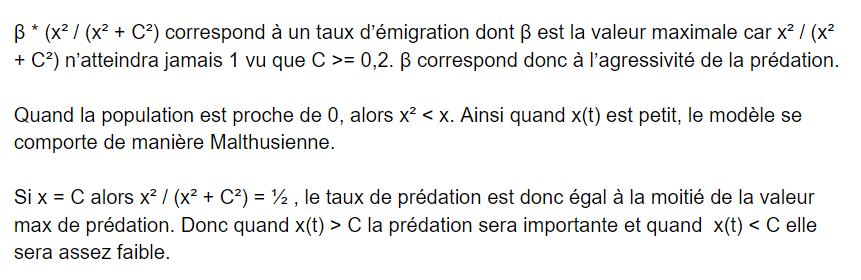
\includegraphics[width=400px]{3.png}
\end{center}

\newpage
\appendix

\section{Etude du modèle logistique avec effet Allee et immigration- Scripts Scilab}

\subsection{Modèle avec variation de I}

\subsubsection{Vitesse d'accroissement}

\begin{verbatim}
clear
clf

r = 0.5 ; A = 0.5 ; K = 2 ; // variables du modèle
Ivect=0:0.1:1; // variable qui varie
x = linspace(0, 2.2, 301); // vecteur contenant les valeurs de la vitesse d'accroissement

function f = allee_imig(x) // fonction qui calcule la vitesse d'accroissement
    f = r * x .* (x / A - 1 ) .* (1 - x / K)+ I // opérations vectorielles. x est un vecteur
endfunction

for i=1:11; // Bouclae qui va dessiner les différentes courbes
    I=Ivect(i); // Assignation valeur qui varie
    plot2d(x, allee_imig(x), style = i) // Tracé de la vitesse d'accroissement
end

// Définition des paramètres d'affichages
a=gca();
a.x_location = "origin";
a.grid=[5,5];
\end{verbatim}

\subsubsection{Discretisation}

\begin{verbatim}
clear
clf

Ivect=0:0.1:1; // variable qui varie
r = 0.5 ; A = 0.5 ; K = 2 ; h = 0.05 ; a = 0.6 ; // variables du modèle + pas de temps
ndate = 0:h:20; // vecteur des instants où on calcule la solution

function f = allee_img(x) // fonction qui calcule la vitesse d'accroissement
    f = r * x .* (x / A - 1 ) .* (1 - x / K)+I // opérations vectorielles. x est un vecteur
endfunction

x(1)=a; // Initialisation de la population initiale

for i=1:11; // Boucle qui va dessiner les différentes courbes
    I=Ivect(i); // Assignation valeur qui varie
    for n = 1:length(ndate) - 1 // Boucle qui calcule la courbe de la population
        x(n+1) = x(n) + h * allee_img(x(n)); // Calcul de la population
    end 
    plot2d(ndate, x, style = i) // Tracé de la discretisation
end

// Définition des paramètres d'affichages
a=gca();
a.x_location = "origin";
a.grid=[5,5];
\end{verbatim}

\subsection{Modèle avec variation de K}

\subsubsection{Vitesse d'accroissement}

\begin{verbatim}
clear
clf

r = 1 ; A = 0.8 ; I=0.05 ; // variables du modèle
Kvect=1.5:0.1:2.5; // variable qui varie
x = linspace(0, 2.2, 301); // vecteur contenant les valeurs de la vitesse d'accroissement

function f = allee_imig(x) // fonction qui calcule la vitesse d'accroissement
    f = r * x .* (x / A - 1 ) .* (1 - x / K)+ I // opérations vectorielles. x est un vecteur
endfunction

for i=1:11; // Boucle qui va dessiner les différentes courbes
    K=Kvect(i); // Assignation valeur qui varie
    plot2d(x, allee_imig(x), style = i) // Tracé de la vitesse d'accroissement
end

// Définition des paramètres d'affichages
a=gca();
a.x_location = "origin";
a.grid=[5,5];
\end{verbatim}

\subsubsection{Discretisation}

\begin{verbatim}
clear
clf

Kvect=1.5:0.1:2.5; // variable qui varie
r = 1 ; A = 0.8 ; I=0.05 ; h = 0.05 ; a = 0.7 ; // variables du modèle + pas de temps
ndate = 0:h:20; // vecteur des instants où on calcule la solution

function f = allee_img(x) // fonction qui calcule la vitesse d'accroissement
    f = r * x .* (x / A - 1 ) .* (1 - x / K)+I // opérations vectorielles. x est un vecteur
endfunction

x(1)=a; // Initialisation de la population initiale

for i=1:11; // Boucle qui va dessiner les différentes courbes
    K=Kvect(i); // Assignation valeur qui varie
    for n = 1:length(ndate) - 1 // Boucle qui calcule la courbe de la population
        x(n+1) = x(n) + h * allee_img(x(n)); // Calcul de la population
    end 
    plot2d(ndate, x, style = i) // Tracé de la discretisation
end

// Définition des paramètres d'affichages
a=gca();
a.x_location = "origin";
a.grid=[5,5];
\end{verbatim}

\subsection{Modèle avec variation de A}

\subsubsection{Vitesse d'accroissement}

\begin{verbatim}
clear
clf

r = 1 ; K = 2 ; I=0.1 ; // variables du modèle
Avect=0.5:0.1:1.5; // variable qui varie
x = linspace(0, 2.2, 301); // vecteur contenant les valeurs de la vitesse d'accroissement

function f = allee_imig(x) // fonction qui calcule la vitesse d'accroissement
    f = r * x .* (x / A - 1 ) .* (1 - x / K)+ I // opérations vectorielles. x est un vecteur
endfunction

for i=1:11; // Boucle qui va dessiner les différentes courbes
    A=Avect(i); // Assignation valeur qui varie
    plot2d(x, allee_imig(x), style = i) // Tracé de la vitesse d'accroissement
end

// Définition des paramètres d'affichages
a=gca();
a.x_location = "origin";
a.grid=[5,5];
\end{verbatim}

\subsubsection{Discretisation}

\begin{verbatim}
clear
clf

Avect=0.5:0.1:1.5; // variable qui varie
r = 1 ; K = 2 ; I=0.1 ; h = 0.05 ; a = 0.7 ; // variables du modèle + pas de temps
ndate = 0:h:20; // vecteur des instants où on calcule la solution

function f = allee_img(x) // fonction qui calcule la vitesse d'accroissement
    f = r * x .* (x / A - 1 ) .* (1 - x / K)+I // opérations vectorielles. x est un vecteur
endfunction

x(1)=a; // Initialisation de la population initiale

for i=1:11; // Boucle qui va dessiner les différentes courbes
    A=Avect(i); // Assignation valeur qui varie
    for n = 1:length(ndate) - 1 // Boucle qui calcule la courbe de la population
        x(n+1) = x(n) + h * allee_img(x(n)); // Calcul de la population
    end 
    plot2d(ndate, x, style = i) // Tracé de la discretisation
end

// Définition des paramètres d'affichages
a=gca();
a.x_location = "origin";
a.grid=[5,5];
\end{verbatim}

\subsection{Modèle avec variation de la population initiale}

\begin{verbatim}
clear
clf

avect=0.2:0.2:2.2; // variable qui varie
r = 0.5 ; K = 2 ; I=0.05 ; A = 0.5 ; h = 0.05 ; // variables du modèle + pas de temps
ndate = 0:h:20; // vecteur des instants où on calcule la solution

function f = allee_img(x) // fonction qui calcule la vitesse d'accroissement
    f = r * x .* (x / A - 1 ) .* (1 - x / K)+I // opérations vectorielles. x est un vecteur
endfunction

for i=1:11; // Boucle qui va dessiner les différentes courbes
    x(1)=avect(i); // Assignation valeur qui varie
    for n = 1:length(ndate) - 1 // Boucle qui calcule la courbe de la population
        x(n+1) = x(n) + h * allee_img(x(n)); // Calcul de la population
    end 
    plot2d(ndate, x, style = i) // Tracé de la discretisation
end

// Définition des paramètres d'affichages
a=gca();
a.x_location = "origin";
a.grid=[5,5];
\end{verbatim}

\section{Etude du modèle logistique avec prédation - Scripts Scilab}

\subsection{Modèle}

\subsubsection{Vitesse d'accroissement}

\begin{verbatim}
clear
clf

// variables du modèle
r = 1 ; A = 0.5 ; K = 2.5 ; B=0.5 ; C=0.3 ;
x = linspace(0, 2.5, 301);

function f = predation(x) // fonction qui calcule la vitesse d'accroissement
    f =r * x .* (1 - x / K) - B * (x.^2 ./ (x.^2 + C^2)) // opération vectorielle
endfunction

plot2d(x, predation(x), style = 2); // Tracé de la vitesse d'accroissement

// Définition des paramètres d'affichages
a=gca();
a.x_location = "origin";
a.grid=[5,5];
\end{verbatim}

\subsubsection{Discretisation}

\begin{verbatim}
clear
clf

// variables du modèle
r = 1 ; A = 0.5 ; K = 2.5 ; B=0.5 ; C=0.4 ; h = 0.05 ; a = 1;
ndate = 0:h:20; // vecteur des instants

function f = predation(x) // fonction qui calcule la vitesse d'accroissement
    f =r * x .* (1 - x / K) - B * (x.^2 ./ (x.^2 + C^2)) // opération vectorielle
endfunction

x(1) = a; // Initialisation de la population initiale

for n = 1:length(ndate) - 1 // Boucle qui calcule la courbe de la population
    x(n+1) = x(n) + h * predation(x(n)); // Calcul de la population
end

plot2d(ndate, x, style = 2) // Tracé de la trajectoire

// Définition des paramètres d'affichages
a=gca();
a.x_location = "origin";
a.grid=[5,5];
\end{verbatim}

\subsection{Modèle avec variation de B}

\subsubsection{Vitesse d'accroissement}

\begin{verbatim}
clear
clf

// variables du modèle
r = 1 ; A = 0.5 ; K = 2.5 ; C=0.4 ;
Bvect = 0.3:0.1:0.7; // variable qui varie
x = linspace(0, 2.5, 301);

function f = predation(x) // fonction qui calcule la vitesse d'accroissement
    f =r * x .* (1 - x / K) - B * (x.^2 ./ (x.^2 + C^2)) // opération vectorielle
endfunction

for i=1:5 // Boucle qui va dessiner les différentes courbes

    B=Bvect(i); // Assignation valeur qui varie

    plot2d(x, predation(x), style = i); // Tracé de la vitesse d'accroissement

end

// Définition des paramètres d'affichages
a=gca();
a.x_location = "origin";
a.grid=[5,5];
\end{verbatim}

\subsubsection{Discretisation}

\begin{verbatim}
clear
clf

Bvect = 0.3:0.1:0.7; // variable qui varie
// variables du modèle
r = 1 ; A = 0.5 ; K = 2.5 ; C=0.4 ; a = 1 ; h = 0.05 ;
ndate = 0:h:20; // vecteur des instants

function f = predation(x) // fonction qui calcule la vitesse d'accroissement
    f =r * x .* (1 - x / K) - B * (x.^2 ./ (x.^2 + C^2)) // opération vectorielle
endfunction

for i=1:5 // Boucle qui va dessiner les différentes courbes
    
    B=Bvect(i); // Assignation valeur qui varie
    x(1) = a; // Initialisation de la population initiale
    
    for n = 1:length(ndate) - 1 // Boucle qui calcule la courbe de la population
        x(n+1) = x(n) + h * predation(x(n)); // Calcul de la population
    end
    
    plot2d(ndate, x, style = i) // Tracé de la trajectoire

end

// Définition des paramètres d'affichages
a=gca();
a.x_location = "origin";
a.grid=[5,5];
\end{verbatim}


\subsection{Modèle avec variation de C}

\subsubsection{Vitesse d'accroissement}

\begin{verbatim}
clear
clf

// variables du modèle
r = 1 ; A = 0.5 ; K = 2.5 ; B=0.5 ;
Cvect = 0.2:0.05:0.4; // variable qui varie
x = linspace(0, 2.5, 301);

function f = predation(x) // fonction qui calcule la vitesse d'accroissement
    f =r * x .* (1 - x / K) - B * (x.^2 ./ (x.^2 + C^2)) // opération vectorielle
endfunction

for i=1:5 // Boucle qui va dessiner les différentes courbes
 
    C=Cvect(i); // Assignation valeur qui varie

    plot2d(x, predation(x), style = i); // Tracé de la vitesse d'accroissement

end

// Définition des paramètres d'affichages
a=gca();
a.x_location = "origin";
a.grid=[5,5];
\end{verbatim}

\subsubsection{Discretisation}

\begin{verbatim}
clear
clf

Cvect = 0.2:0.05:0.4; // variable qui varie
// variables du modèle
r = 1 ; A = 0.5 ; K = 2.5 ; B=0.5 ; h = 0.05 ; a = 0.3 ;
ndate = 0:h:20; // vecteur des instants

function f = predation(x) // fonction qui calcule la vitesse d'accroissement
    f =r * x .* (1 - x / K) - B * (x.^2 ./ (x.^2 + C^2)) // opération vectorielle
endfunction

for i=1:5 // Boucle qui va dessiner les différentes courbes
    
    C=Cvect(i); // Assignation valeur qui varie
    x(1) = a; // Initialisation de la population initiale
    
    for n = 1:length(ndate) - 1 // Boucle qui calcule la courbe de la population
        x(n+1) = x(n) + h * predation(x(n)); // Calcul de la population
    end
    
    plot2d(ndate, x, style = i) // Tracé de la trajectoire

end

// Définition des paramètres d'affichages
a=gca();
a.x_location = "origin";
a.grid=[5,5];
\end{verbatim}

\subsection{Modèle avec variation de la population initiale}

\subsubsection{Discretisation}

\begin{verbatim}
clear
clf

avect= 0.5:0.5:3.5; //vecteur des différentes valeurs de a
// variables du modèle
r = 1 ; A = 0.5 ; K = 2.5 ; B=0.5 ; C=0.4 ; h = 0.05 ; I=0.2 ;
ndate = 0:h:20; // vecteur des instants


function f = predation(x) // fonction du modèle logistique avec effet de prédation
    f =r * x .* (1 - x / K) - B * (x.^2 ./ (x.^2 + C^2)) // opération vectorielle
endfunction

for i=1:7 // Boucle qui va dessiner les différentes courbes
    a=avect(i); // Assignation valeur qui varie
    x(1) = a; // Initialisation de la population initiale
    for n = 1:length(ndate) - 1 // Boucle qui calcule la courbe de la population
        x(n+1) = x(n) + h * predation(x(n)); // Calcul de la population
    end
    plot2d(ndate, x, style = i) // Tracé de la courbe
end

// Définition des paramètres d'affichages
z=gca();
z.x_location = "origin";
z.grid=[5,5];
\end{verbatim}

\end{document}